W tym podrozdziale przyjrzymy się, jak poszczególne moduły gry ze sobą współpracują na podstawie załączonego diagramu. Zobaczysz, jakie interakcje zachodzą między różnymi częściami projektu, jak są przekazywane informacje oraz w jaki sposób poszczególne moduły komunikują się ze sobą, by zapewnić spójność i płynność działania gry.
\begin{figure}[h]
    \centering
    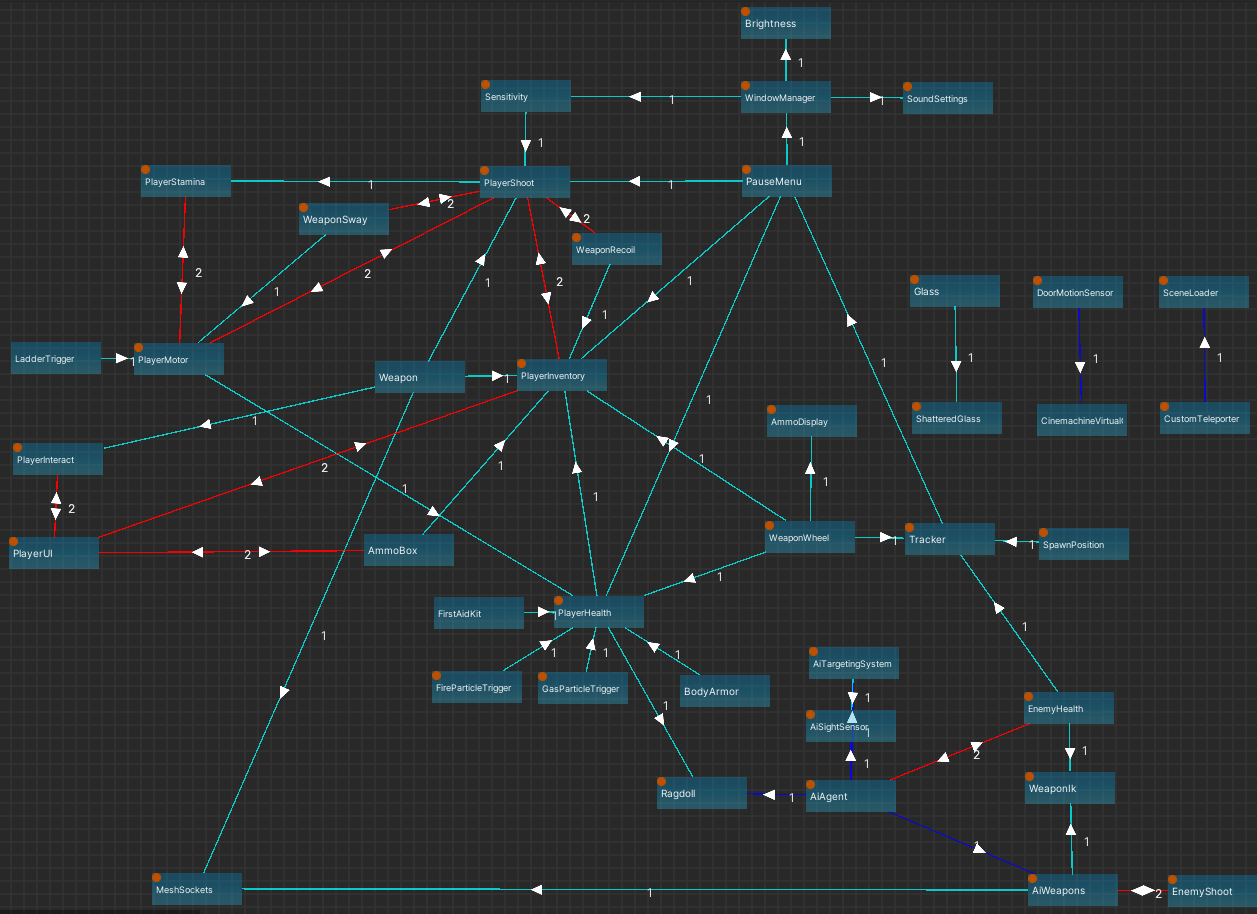
\includegraphics[width=1\linewidth]{Images/modulesDependency.png}
    \caption{Komunikacja między modułami}
\end{figure}
\FloatBarrier